%!TEX root = main-doc.tex
%
% File: background.tex
%
% Date: ? 
%
% Description:
%   The background is given to ...
%
%
\chapter{Background} \label{chap:background}
\vspace{-1cm}
\summary{This chapter provides a background on data warehousing and OLAP, extendible multidimensional dense arrays and multidimensional sparse arrays.}

%%%%%%%%%%%%%%%%%%%%%%%%%%%%%%%%%%%%%%%%%%%%%%%%%%%%%%%%%%%%%%%%%%%%%%%%%%%%%%%%
\section{Data Warehousing}
In Chapter \ref{chap:introduction} it was discovered how important information is in the current world \cite{golfarelli:2009:dwd}. It was also discussed that due to the vast amounts of data being created and stored every day and the inability for traditional database methods (e.g. SQL database systems) to deal with such large volumes of data, data warehousing was created for decision making.

Bill Inmon defines data warehousing as an architecture that is a subject-oriented, non-volatile, integrated, time variant collection of data created for the purpose of management’s decision making. 

Ralph Kimball defines a data warehouse as a copy of transaction data specifically structured for query and analysis.

The modern advanced data warehousing processes allow for OLAP by creating a new data repository that integrates basic data from various sources, arranges the data formats and makes the data available for analysis and decision-making \cite{golfarelli:2009:dwd}. OLAP queries require dynamic, multidimensional analyses of huge quantities of data to process records for decision-making. OLAP queries make use of multidimensional representations of data warehouses as the data is viewed as points in space whose dimensions correspond to many possible analysis dimensions \cite{golfarelli:2009:dwd}. A 3D data warehouse cube is given in Figure \ref{fig:exampleCube} to explicitly show why multidimensional representations are important for OLAP.

 \begin{figure}[H]
	\centering
	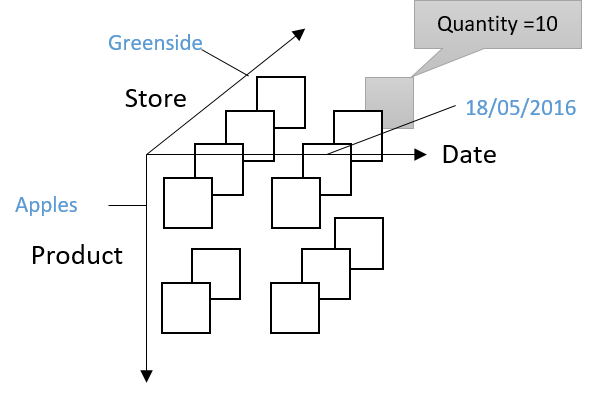
\includegraphics[width=0.6\linewidth]{exampleCube}
	\caption{An Example of a Multidimensional Data Warehouse}
	\label{fig:exampleCube}
\end{figure}

The data warehousing and OLAP operations that are most commonly used include: Get, Insert, Addition, Multiplication, Subtraction, Division, roll-up, drill-down, slice-and-dice, pivot, drill-across, drill-through, and range or box access.

%%%%%%%%%%%%%%%%%%%%%%%%%%%%%%%%%%%%%%%%%%%%%%%%%%%%%%%%%%%%%%%%%%%%%%%%%%%%%%%%
\section{Methodologies}
In order to develop a model for extendible multi-dimensional sparse arrays, the current representations of extendible multi-dimensional arrays must be analysed. The study of the current representations will give a clear indication of how to integrate the representation of extendible multi-dimensional sparse arrays, so that the model can easily be integrated into the current system, preventing unnecessary additional costs. Once a model has been developed, compression of data as well as computing speed will be assessed.

%%%%%%%%%%%%%%%%%%%%%%%%%%%%%%%%%%%%%%%%%%%%%%%%%%%%%%%%%%%%%%%%%%%%%%%%%%%%%%%%
\section{Sparse Array Representations}
There are numerous studies that have been conducted on the efficiency of different sparse array representation schemes \cite{wang:2014sar,goil:bess}. In order to accurately understand these models, we must first understand exactly what is mean by a sparse array. If an array is sparse, it has very few non-zero elements relative to the product of the cardinalities \cite{wang:2014sar}.

There are three main methods used for 2-dimensional sparse array representations, namely: 
\begin{enumerate}
	\item Matrix Market (known as a relational table or a Triplicate)
	\item Linked list
	\item Compressed Row (or alternatively Column) Storage (CRS/CCS)
\end{enumerate}	

There are six other methods that are used for multidimensional representations, namely: 
\begin{enumerate}
	\item Bit-Encoded Sparse Storage (BESS) 
	\item Extended CRS/CCS known as xCRS and xCCS
	\item PATRICIA Trie Compressed Storage (PTCS)
	\item Bit-Encoded Compressed Row (or Column) storage (BxCRS/BxCCS)
	\item Hybrid approach (Hybrid) that combines BESS with xCRS
\end{enumerate}

BESS is the simplest low level storage scheme that chops every point into bit block dimensions. BESS has decent storage, but is traditionally static with the maximum number of chunks being determined algorithmically.

The PTCS is unique and allows for extendibility with regards to data warehousing operations.

%%%%%%%%%%%%%%%%%%%%%%%%%%%%%%%%%%%%%%%%%%%%%%%%%%%%%%%%%%%%%%%%%%%%%%%%%%%%%%%%
%\section{Dynamic Sparse Arrays}
%Increasing Density
%\begin{itemize}
%	\item Bounds and structure remain the same
%	\item new elements are slot into a chunk where there was a free space
%\end{itemize}
%Increasing Bound

%%%%%%%%%%%%%%%%%%%%%%%%%%%%%%%%%%%%%%%%%%%%%%%%%%%%%%%%%%%%%%%%%%%%%%%%%%%%%%%%
\section{Big Data Representations}

Big Data characterization
\begin{itemize}
	\item Volume - Scalability, storage to grow - investigate using a parallel file system
	\item Velocity - Cope with speed, rate at which data comes in - times series
	\item Variety - Data types - different formats i.e multimedia databases for geographic location - GI, Spacial, Moving Targets, structured, unstructured/text, legal documents - Databases that capture almost everything.
	\item Veracity - validity
	\item Value
	%\item Fault tolerance must be researched 
\end{itemize}

\begin{itemize}
	\item Capable of holding very large amounts of data.
	\item Hold the data in inexpensive storage devices.
	\item Processing is done by the “Roman census” method.
	\item Data is stored in an unstructured format.
	\item Hierarchical Data Format (HDF5)
	\begin{itemize}
		\item Data model, library, and file format for storing and managing data
		\item Supports an unlimited variety of datatypes, and is designed for flexible and efficient I/O and for high volume and complex data. 
		\item Portable and extensible, allowing applications to evolve in their use of HDF5.
		\item Tools and applications for managing, manipulating, viewing, and analyzing data in the HDF5 format. 
		\item Organized in a hierarchical structure, with two primary structures: groups and datasets. 
		\begin{itemize}
			\item group: a grouping structure containing instances of zero or more groups or datasets, together with supporting metadata. 
			\item dataset: a multidimensional array of data elements, together with supporting metadata. 
		\end{itemize}
	\end{itemize}
	\item Hadoop
	\begin{itemize}
		\item Distributed storage and processing of very large data sets. 
		\item Consists of computer clusters built from commodity hardware.
		\item Assumption that hardware failures are common occurrences and should be automatically handled by the framework
		\item Hadoop can run parallel queries over flat files. This allows it do basic operational reporting on data in its original form.
		\item Hadoop splits files into large blocks and distributes them across nodes in a cluster. It then transfers packaged code into nodes to process the data in parallel
		\item Hadoop framework includes following four modules:
		\begin{itemize}
			\item Hadoop Common: These libraries provides filesystem and OS level abstractions and contains the necessary Java files and scripts required to start Hadoop.
			\item Hadoop YARN: This is a framework for job scheduling and cluster resource management.
			\item Hadoop Distributed File System (HDFS™): A distributed file system that provides high-throughput access to application data.
			\item Hadoop MapReduce: This is YARN-based system for parallel processing of large data sets.
		\end{itemize}
	\end{itemize}
	\item Network Common Data Form (NetCDF)
	\begin{itemize}
		\item Set of software libraries and self-describing, machine-independent data formats that support the creation, access, and sharing of array-oriented scientific data.
	\end{itemize}
\end{itemize}

%%%%%%%%%%%%%%%%%%%%%%%%%%%%%%%%%%%%%%%%%%%%%%%%%%%%%%%%%%%%%%%%%%%%%%%%%%%%%%%%
\section{TileDB storage manager}
\begin{itemize}
	\item Used for data which is represented as multi-dimensional arrays.
	\item Sparse arrays significantly impact storage and application performance
	\item when storing data cells that are accessed together should be co-located -  global cell orders in data tiles in sparse arrays include row-major vs column-major
	\item bookkeeping is very important for locating the correct data as exact distribution of the non-empty cells is unknown
	%\item Still working on understanding the internals and basic operations in more depth
	%\item Downloaded some files on reading/writing to sparse arrays (C) - DBexamples on Github - Intel HCS compiler - link between FPGA and GPU
\end{itemize}

%%%%%%%%%%%%%%%%%%%%%%%%%%%%%%%%%%%%%%%%%%%%%%%%%%%%%%%%%%%%%%%%%%%%%%%%%%%%%%%%
%\section{FGPAs}
%Integrated circuit consisting of an array of identical logic blocks with programmable interconnections.
%-I do not feel that FGPAs would be the best suited for the research. \cite{roth:2016:dsd}

%%%%%%%%%%%%%%%%%%%%%%%%%%%%%%%%%%%%%%%%%%%%%%%%%%%%%%%%%%%%%%%%%%%%%%%%%%%%%%%%
\section{Impact}

%%%%%%%%%%%%%%%%%%%%%%%%%%%%%%%%%%%%%%%%%%%%%%%%%%%%%%%%%%%%%%%%%%%%%%%%%%%%%%%%
\section{New Results}
